\documentclass[11pt]{beamer}

\usepackage{url}
\usepackage{tikz}
\author{Armijn Hemel\\Tjaldur Software Governance Solutions}
\title{Computing the license of a binary by tracing build outputs}
\date{April 10, 2014}

\begin{document}

\setlength{\parskip}{4pt}

\frame{\titlepage}

\frame{
\frametitle{About Armijn}
\begin{itemize}
\item owner Tjaldur Software Governance Solutions
\item creator of Binary Analysis Tool (BAT)
\end{itemize}
}

\frame{
\frametitle{About this presentation}
This presentation builds upon earlier work done by:

Eelco Dolstra, Julius Davies, Sander van der Burg, Daniel German and Armijn Hemel

Results were published as a technical report from Delft University of Technology
(TUD SERG 2012-010).

Reworking the prototype tools is still ``work in progress''. Tools will eventually
be part of BAT under Apache 2 license.
}

\frame{
\frametitle{Today's problem}
The question ``What license is this binary under?'' is not as straightforward
as most people think and most people get it \textit{wrong}.
}

\frame{
\frametitle{Example: \texttt{opkg}}
\texttt{opkg} is a package manager that is used on embedded Linux distributions.

Question: given you build \texttt{opkg}, what license(s) can the binary you
built be distributed under?

Hint: Ohloh says \texttt{opkg} is GPLv2.
}

\frame{
\frametitle{GPLv2? GPLv2+? GPLv3+?}
(Note: this applies only to an older but widely used version of \texttt{opkg})

\texttt{opkg} has a \texttt{COPYING} file containing the text of GPLv2.

All source code files in \texttt{opkg} are GPLv2+ \textbf{except} \texttt{libopkg/sha256.c} and \texttt{libopkg/sha256.h} which are GPLv3+!

These files are not always included, but they are most of the time. The \texttt{configure} script has a switch:

\texttt{\\   --enable-sha256         Enable sha256sum check [default=yes]\\}

Correct answer: it depends and more information about the \textit{composition} of the binary is needed.
}

\begin{frame}[fragile]
\frametitle{Example: MUNGE}
\begin{verbatim}
MUNGE is free software: you can redistribute it and/or
modify it under the terms of the GNU General Public
License as published by the Free Software Foundation,
either version 3 of the License, or (at your option)
any later version.  Additionally for the MUNGE library
(libmunge), you can redistribute it and/or modify it
under the terms of the GNU Lesser General Public License
as published by the Free Software Foundation, either
version 3 of the License, or (at your option) any later
version.
\end{verbatim}

But what goes into \texttt{libmunge}?
\end{frame}

\frame{
\frametitle{Why source code scanning is not good enough}
Static analysis (source code level) can tell you a lot, but information is vastly incomplete:

\begin{itemize}
\item many different types of build systems and scripts
\item output from \texttt{configure} has huge influence
\item environment variables set by scripts or users
\item \textit{external dependencies} might not be obviously declared
\end{itemize}

There are many factors that can influence a build which you simply
cannot find out by just scanning the source tree.
}

\frame{
\frametitle{Why binary scanning is not good enough}
Composition is a lot easier to find out with a binary scanner, but:

\begin{itemize}
\item compiler throws away a lot of very useful information (like license headers!)
\item binary analysis tools like BAT work by making an educated \textit{guess} using fingerprinting to find out what was used. There could be false positives/false negatives.
\end{itemize}

Basically by just looking at the binary you ignore a lot of very essential information that you already have access to!
}

\frame{
\frametitle{Now what?}
Source code scanning is not good enough to find out about \textit{composition} but has a lot of information, binary scanning works with incomplete information but can find out about composition.

Best of both worlds: find out about composition and also use information from the source code.
}

\frame{
\frametitle{Solution: tracing the build}
We can track system calls using \texttt{strace} and see which files are used and modified by a build process!

\begin{itemize}
\item no need to modify existing build tools
\item (pretty much) standard package for Linux
\item build system agnostic
\item no special privileges needed
\end{itemize}
}

\begin{frame}[fragile]
\frametitle{Trace example output}
\begin{verbatim}
...
  open("patchelf.cc", O_RDONLY)
  open("/usr/include/c++/4.5.1/string",
    O_RDONLY|O_NOCTTY)
  open("elf.h", O_RDONLY)
...
\end{verbatim}
\end{frame}

\begin{frame}[fragile]
\frametitle{Result: build graph}

\includegraphics[width=1.0\columnwidth]{example}
\end{frame}

\frame{
\frametitle{Pruning the result graph}
Only tracing which files are used gives a \textit{conservative} estimate of which files are used.

False positives (files that are opened, but not used for building the actual binary) can be pruned by using a bit more intelligence.
}

\frame{
\frametitle{Early success: \texttt{FFmpeg}}
\texttt{FFmpeg} is a mix of GPLv2+ and LGPLv2.1+ licensed code. The \texttt{configure} script has an option to only use the LGPLv2.1+ sources for a build.

With our approach we found that some GPLv2+ code was \textit{always} included in \texttt{libavfilter}.

The offending code was in \texttt{libavfilter/x86/gradfun.c}, licensed under the GPLv2+.

This was not trivial to find out from the \texttt{FFmpeg} build scripts.

\texttt{FFmpeg} fixed it within hours after being informed.
}

\begin{frame}[fragile]
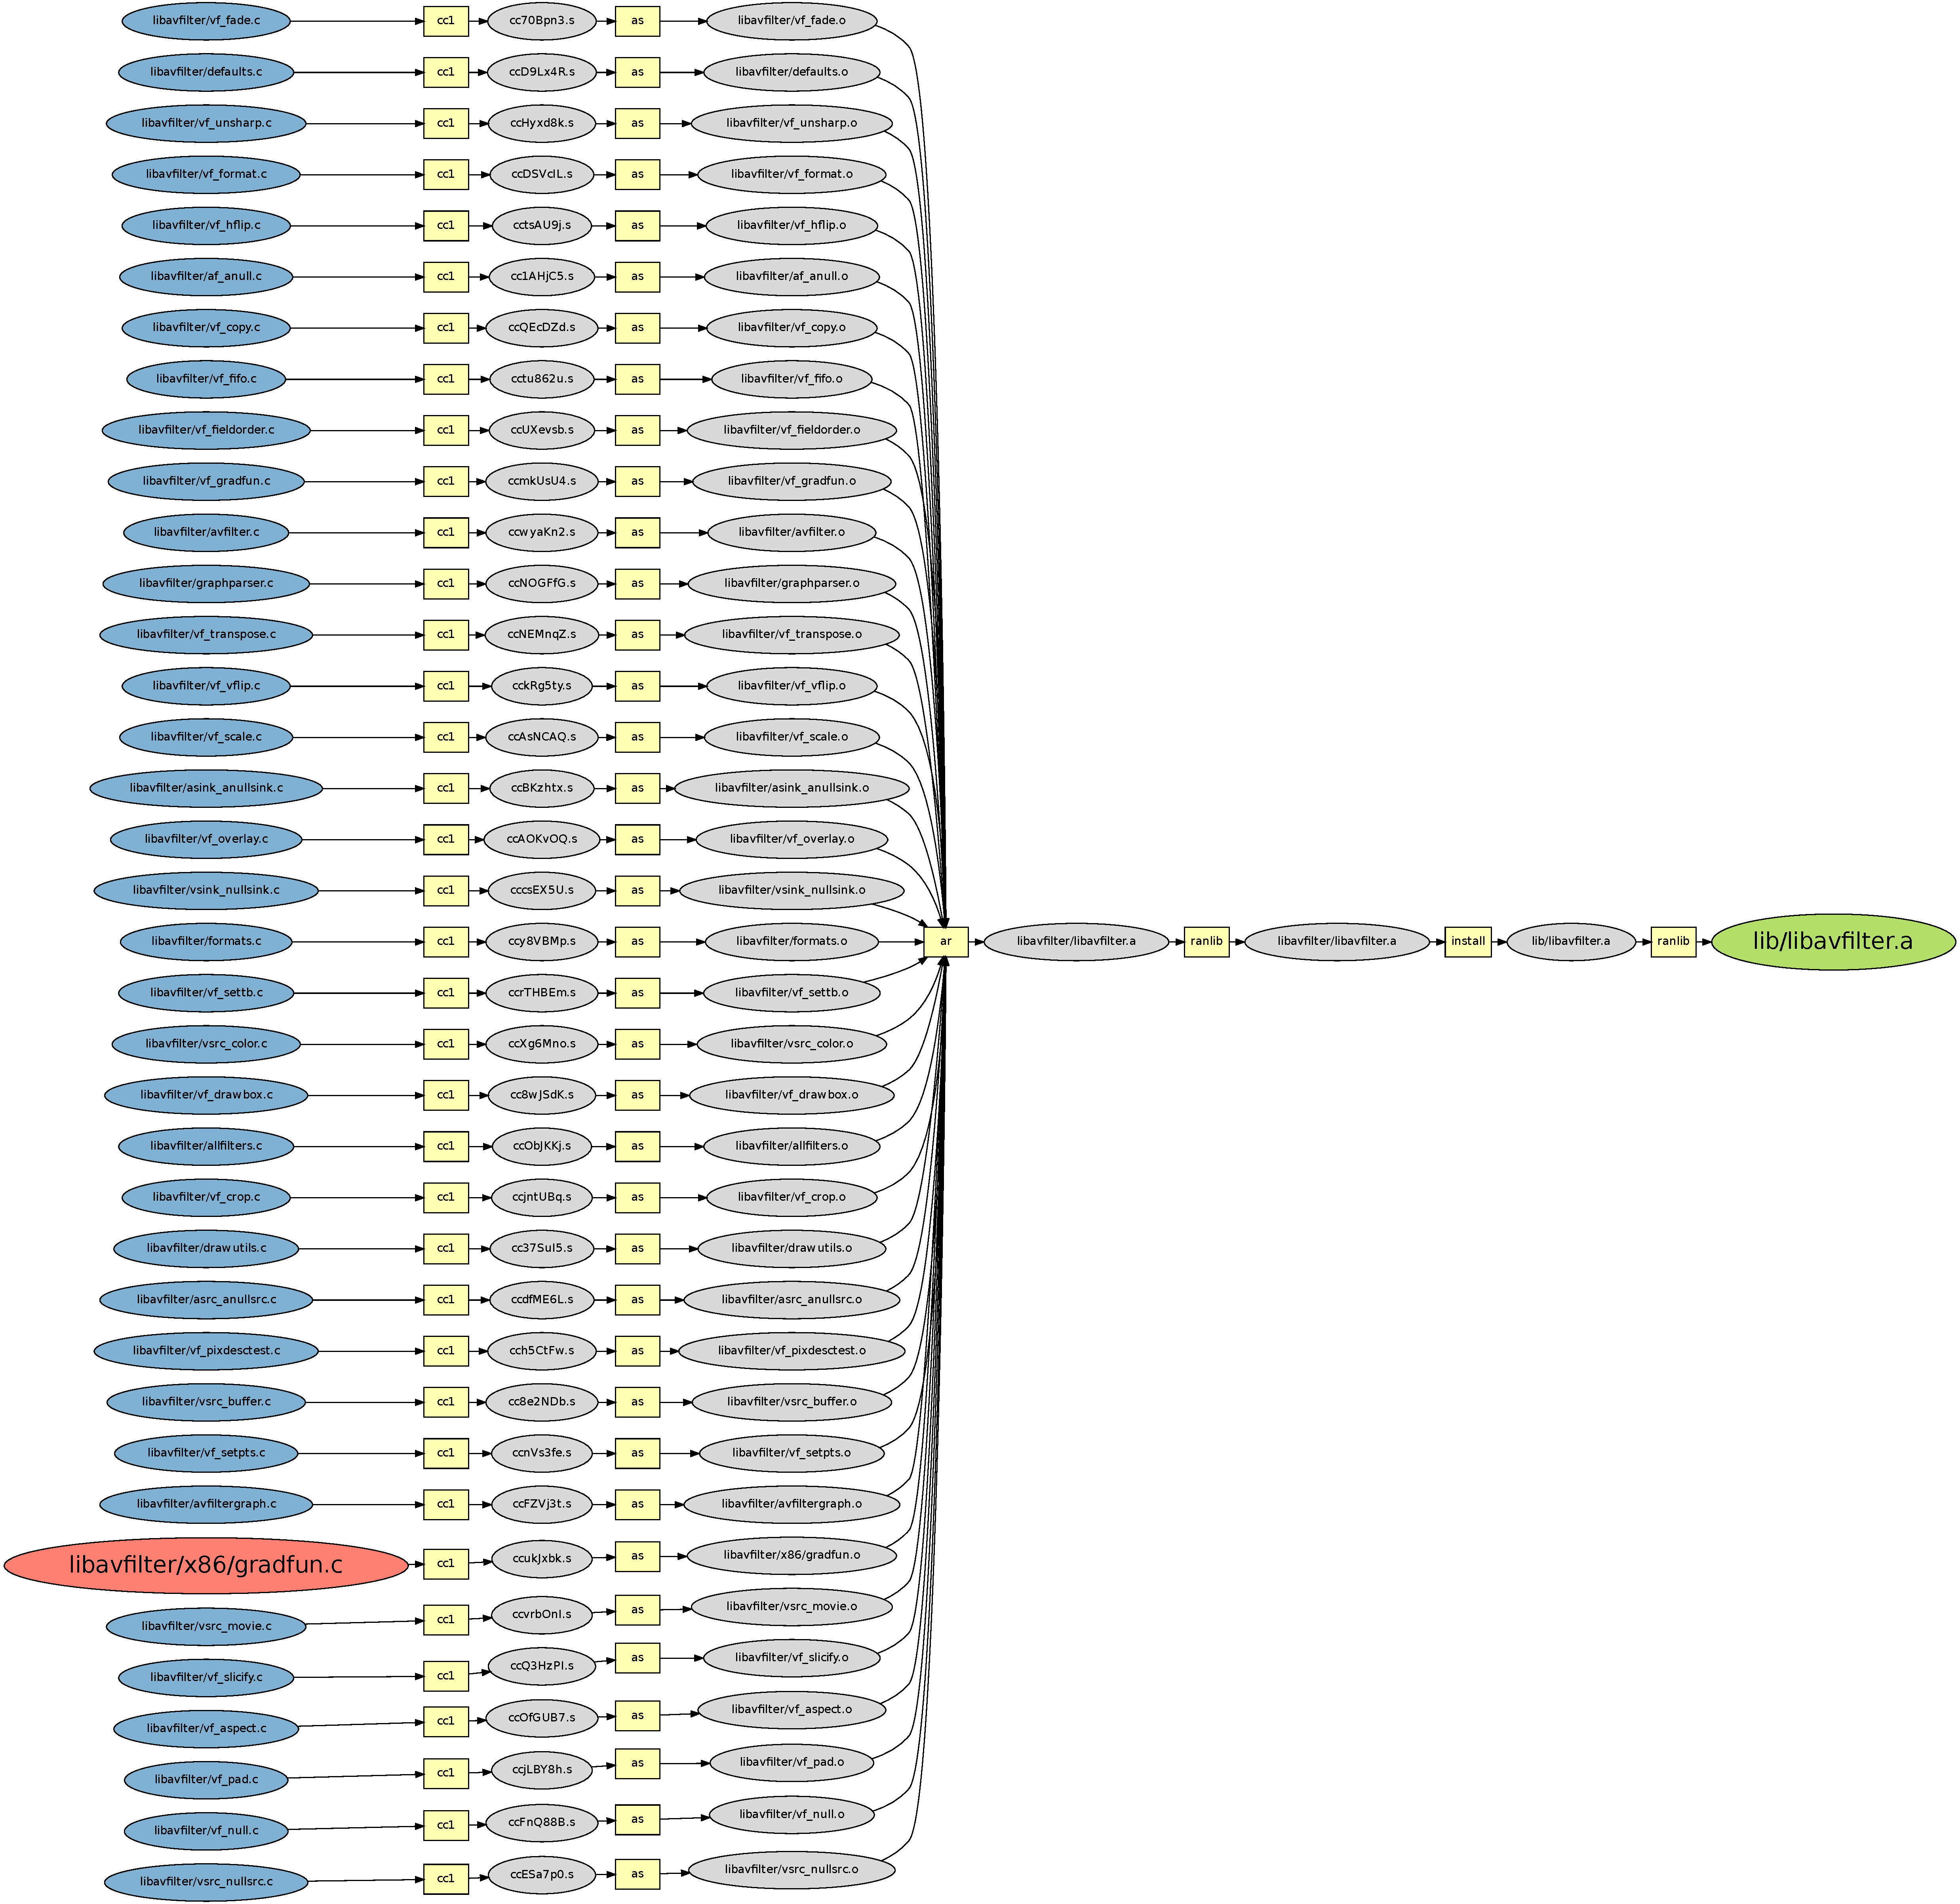
\includegraphics[width=0.9\columnwidth]{ffmpeg_no_gpl_libavfilter_crop}
\end{frame}

\frame{
\frametitle{Drawback: information overload and performance hit}
\texttt{strace} can be \textit{very} verbose and log files (the way I generate them to get enough information) easily can become a few GiB of data.

Tracing also has a significant performance hit so it is not something you want to do every single build.
}

\frame{
\frametitle{Drawback: not all build systems are suitable}
Not all build systems are suitable to be traced, since they open all files in a directory (Java).

In practice I have limited it to C/C++ programs on Linux/*BSD (but it does not always work).

Worst case: all files in the directory tree are seen as input (which is the same as the best
that source code scanners do now).
}

\frame{
\frametitle{Propagating information through the graph}
By adding information to the graph interesting patterns can become visible:

\begin{itemize}
\item security: does this binary include a file with a known security defect?
\item license information: which licenses are combined in the binary?
\end{itemize}
}

\frame{
\frametitle{A license calculus}
By adding licensing information interaction between licenses becomes more visible.

Using simple ``license math'' and rewrite rules we could possible compute a license of a binary!

$BSD2 \rightarrow permissive$\\
$MIT \rightarrow permissive$\\
$GPLv2 + GPLv2orlater = GPLv2$\\
$GPLv2orlater + GPLv3 = GPLv3$\\
$GPLv2 + GPLv3 = error$\\
$permissive + GPLv3orlater = GPLv3orlater$\\
$...$
}

\frame{
\frametitle{A possible basis for a license calculus: ``Linking Document''}
A few years ago a lot of time and effort was sunk into the ``linking document''.
This could (partially) be used as a basis for a calculus.

Some interactions might not be possible to compute or detect automatically,
but I think we can get very far, which is better than what we have today.
}

\frame{
\frametitle{Problem: quality of licensing information}
The method described only works if license information in files is of good quality.
Often licensing information is complete crap.

I use FOSSology and Ninka, which only agree in about 65\% of files I have scanned with
these two scanners because license scanning is \textit{hard}.

(Validos anyone?)
}

\frame{
\frametitle{Current status}
Rough prototype exists, database with licensing information exists,
but I need time to tie everything together.
}

\frame{
\frametitle{Q\&A and discussion}
}

\end{document}
